\ylDisplay{Rong} % Ülesande nimi
{Koit Timpmann} % Autor
{lõppvoor} % Voor
{2019} % Aasta
{P 22} % Ülesande nr.
{2} % Raskustase
{
% Teema: Mehaanika
\ifStatement
Paigalseisust liikuma hakanud raske kaubarong suurendab ühtlaselt kiirust. Pärast esimese $1000$ meetri läbimisel on rong saavutanud kiiruse $v = 10,0$ $m/s$. Kui palju suureneb rongi kiirus teisel kilomeetril?
\fi


\ifHint
Ülesande lahendamisele aitab kaasa kiiruse ja aja vahelist seost kuvava graafiku joonistamine. Kiiruse graafikul on keha poolt läbitud tee võrdne graafiku aluse pindalaga.
\fi

\ifSolution
Kuna rong kiirendas ühtlaselt, siis oli rongi keskmine kiirus esimese kilomeetri läbimisel
\begin{center}
$v = \frac{v_0 + v_1}{2} = 5$ m/s
\end{center}
Seega rong läbis esimese kilomeetri ajaga 
\begin{center}
$t_1 = \frac{s}{v} = 200$ s.
\end{center}
\begin{center}
	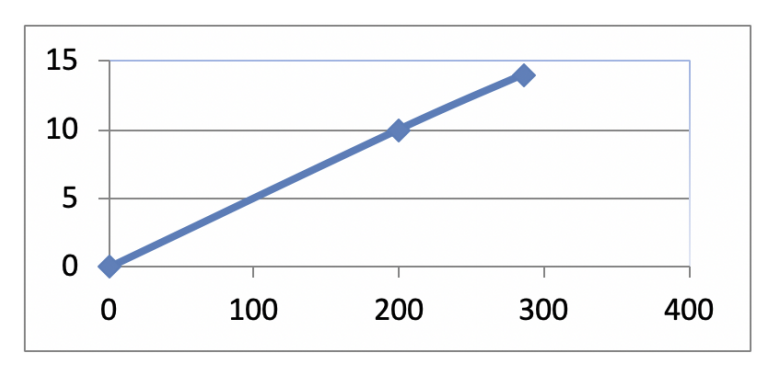
\includegraphics[width=0.5\linewidth]{2019-v3p-22-lah.PNG}
\end{center}
Kiiruse graafikul on keha poolt läbitud tee võrdne graafiku aluse pindalaga. Seega saame kirjutada üles kaks seost kolmnurkade pindalade kaudu.
\begin{center}
$\frac {v1 \cdot t1}{2} = s$ ning $\frac {v2 \cdot t2}{2} = 2s$.
\end{center}
Graafikualused kolmnurgad, mis tekivad 1 km ja 2 km läbimisel on sarnased. Seega saame kirja panna seose
\begin{center}
$\frac{v_2}{v_1} = \frac{t_2}{t_1} \Rightarrow $ $t_2 = \frac{v2 \cdot t1}{v1} $
\end{center}
Asendades selle teise seosesse, saame
\begin{center}
$\frac{v_2 \cdot v_2 \cdot t_1}{2 v_1} = 2s \Rightarrow v_2^2 = \frac{200 m^2}{s^2} \Rightarrow v = 14,1$ m/s. 
\end{center}
Kuna esimese kilomeetri lõpus oli rongi kiiruse 10 m/s, siis kiirus muutus
\begin{center}
$14,1$ m/s $-$ $10$ m/s = $4,1$ m/s.
\end{center}
\fi
}